\documentclass{article}
\usepackage{tikz}
\usetikzlibrary{arrows,decorations.pathmorphing,backgrounds,positioning,fit,petri}
\begin{document}
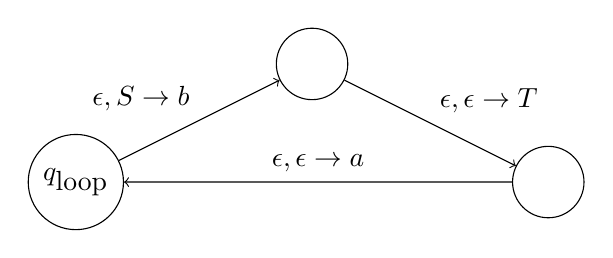
\begin{tikzpicture}[scale=3,
   state/.style={circle, radius=0.14},
   final/.style={radius=0.18}]
   \node (q0) at (1,1) [draw, state] {$q_\textrm{loop}$};

   \node (q1) at (2,1.5) [draw, state] {\phantom{$q_\textrm{lp}$}};
   \node (q2) at (3,1) [draw, state] {\phantom{$q_\textrm{lp}$}};
   \draw (q0)[->] -- node[above left]{$\epsilon,S\to b$} (q1);
   \draw (q1)[->] -- node[above right]{$\epsilon,\epsilon\to T$} (q2);
   \draw (q2)[->] -- node[above]{$\epsilon,\epsilon\to a$} (q0);
\end{tikzpicture}
\end{document}
